\chapter{Antecedentes}

\section{Historia Clinica}

Actualmente en la mayoria de los centros de salud la informacion que compone
la Historias Clinicas de cada paciente es almacenan mediante documentos fisicos,
en su mayoria totalmente elaborados a mano, en otros casos usando plantillas
con campos preformateados (Como se puede Observar en las Figuras 3.1 y 3.2),
lo cual genera varios problemas.\\[0.1cm]

En cuanto al software existente aplicado a la manipulacion de historia clinica,
este suele ser muy incompleto y abocado a la especialidad del medico, es por
ello que si esta informatizado cada area suele manejar sistemas que terminan
siendo incompatibles entre si.\\[0.1cm]

\begin{figure}[h]
    \centering
    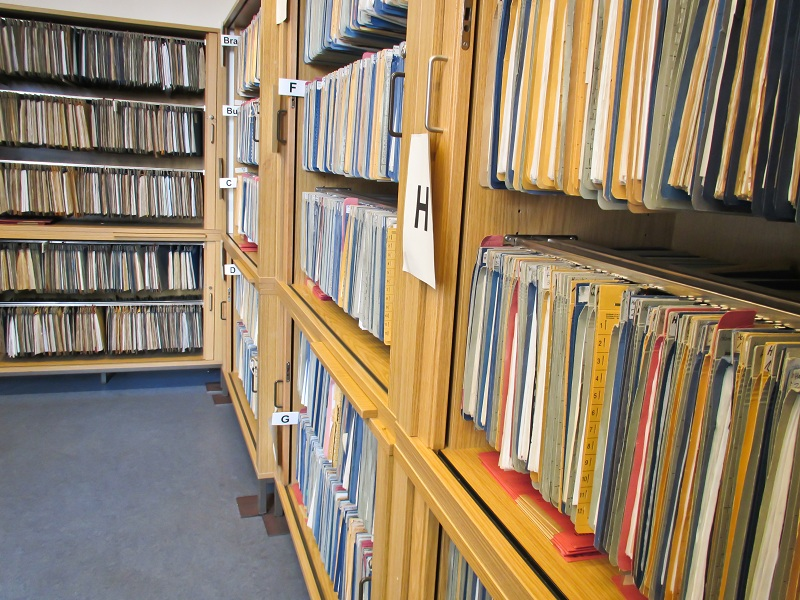
\includegraphics[scale=1.5]{resourse/folders-archivos.jpg}
    \caption{Almacenamiento Fisico de Archivos}
    \label{fig:05}
\end{figure}  


\begin{figure}[H]
    \centering
    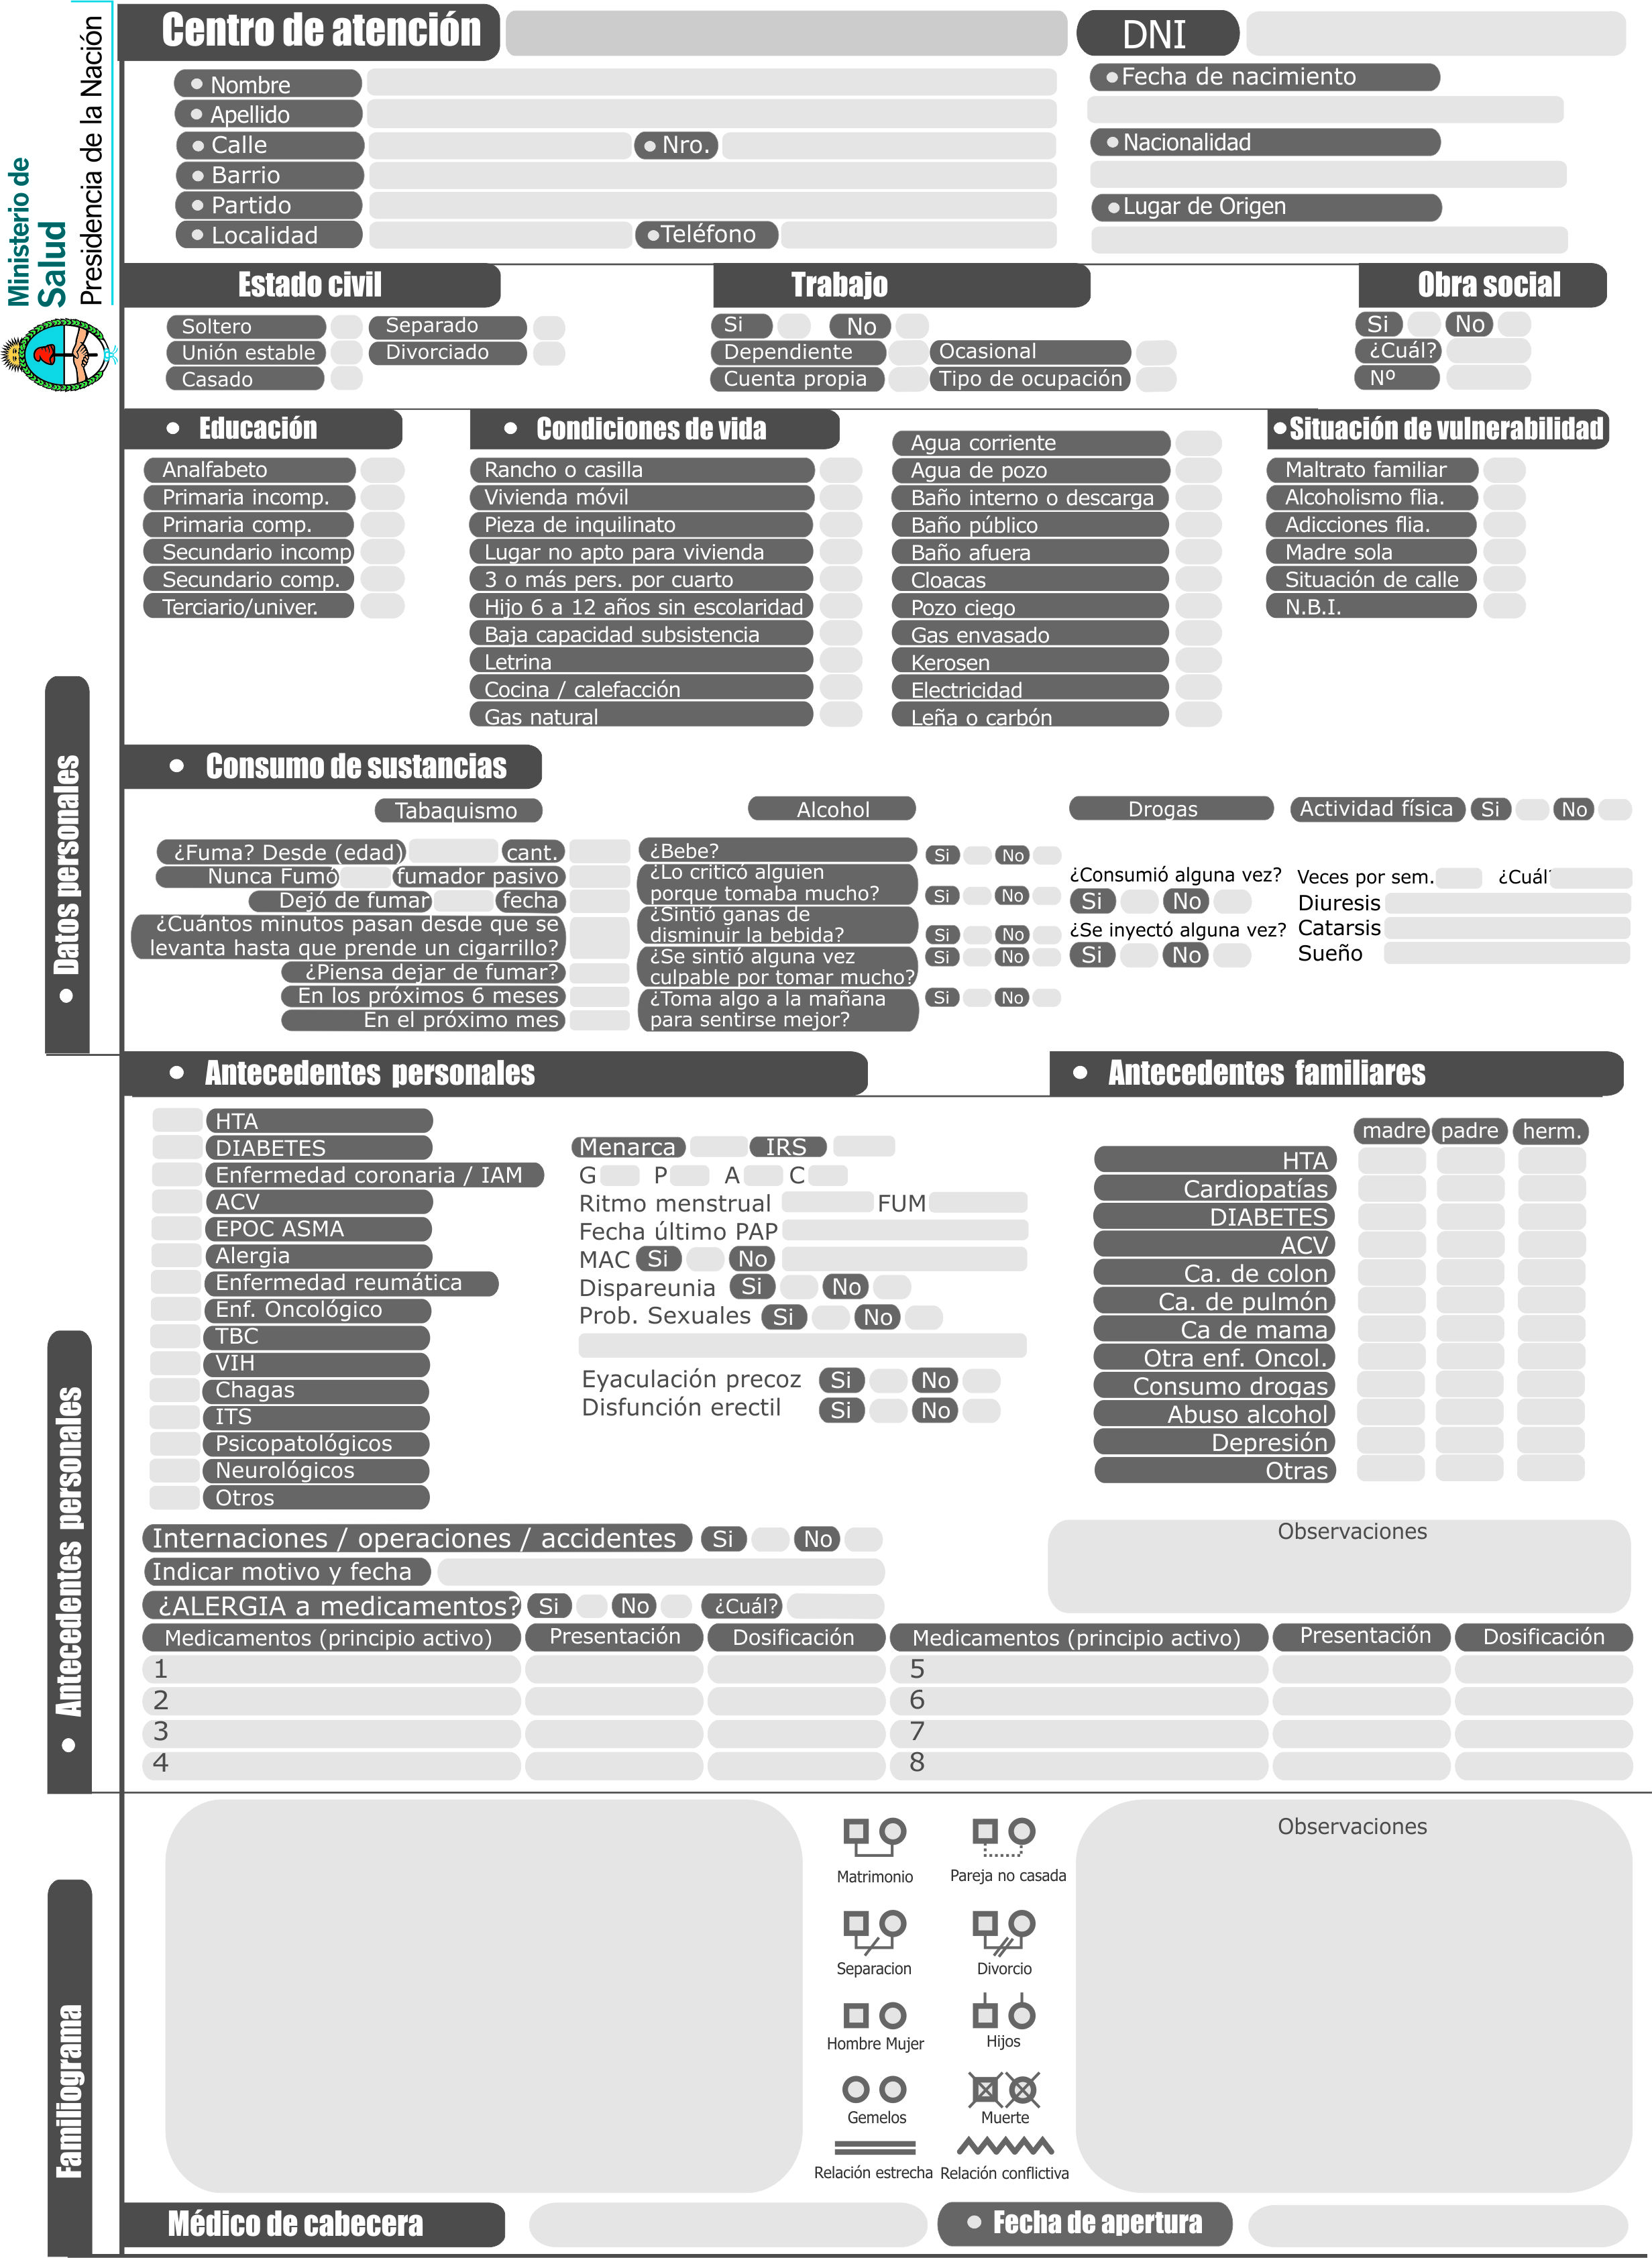
\includegraphics[scale=0.7]{resourse/historia-clinica-f.jpg}
    \caption{Modelo Historia Clinica Ministerio de Salud de La Nacion Pag 1}
    \label{fig:06}
\end{figure}  

\begin{figure}[H]
    \centering
    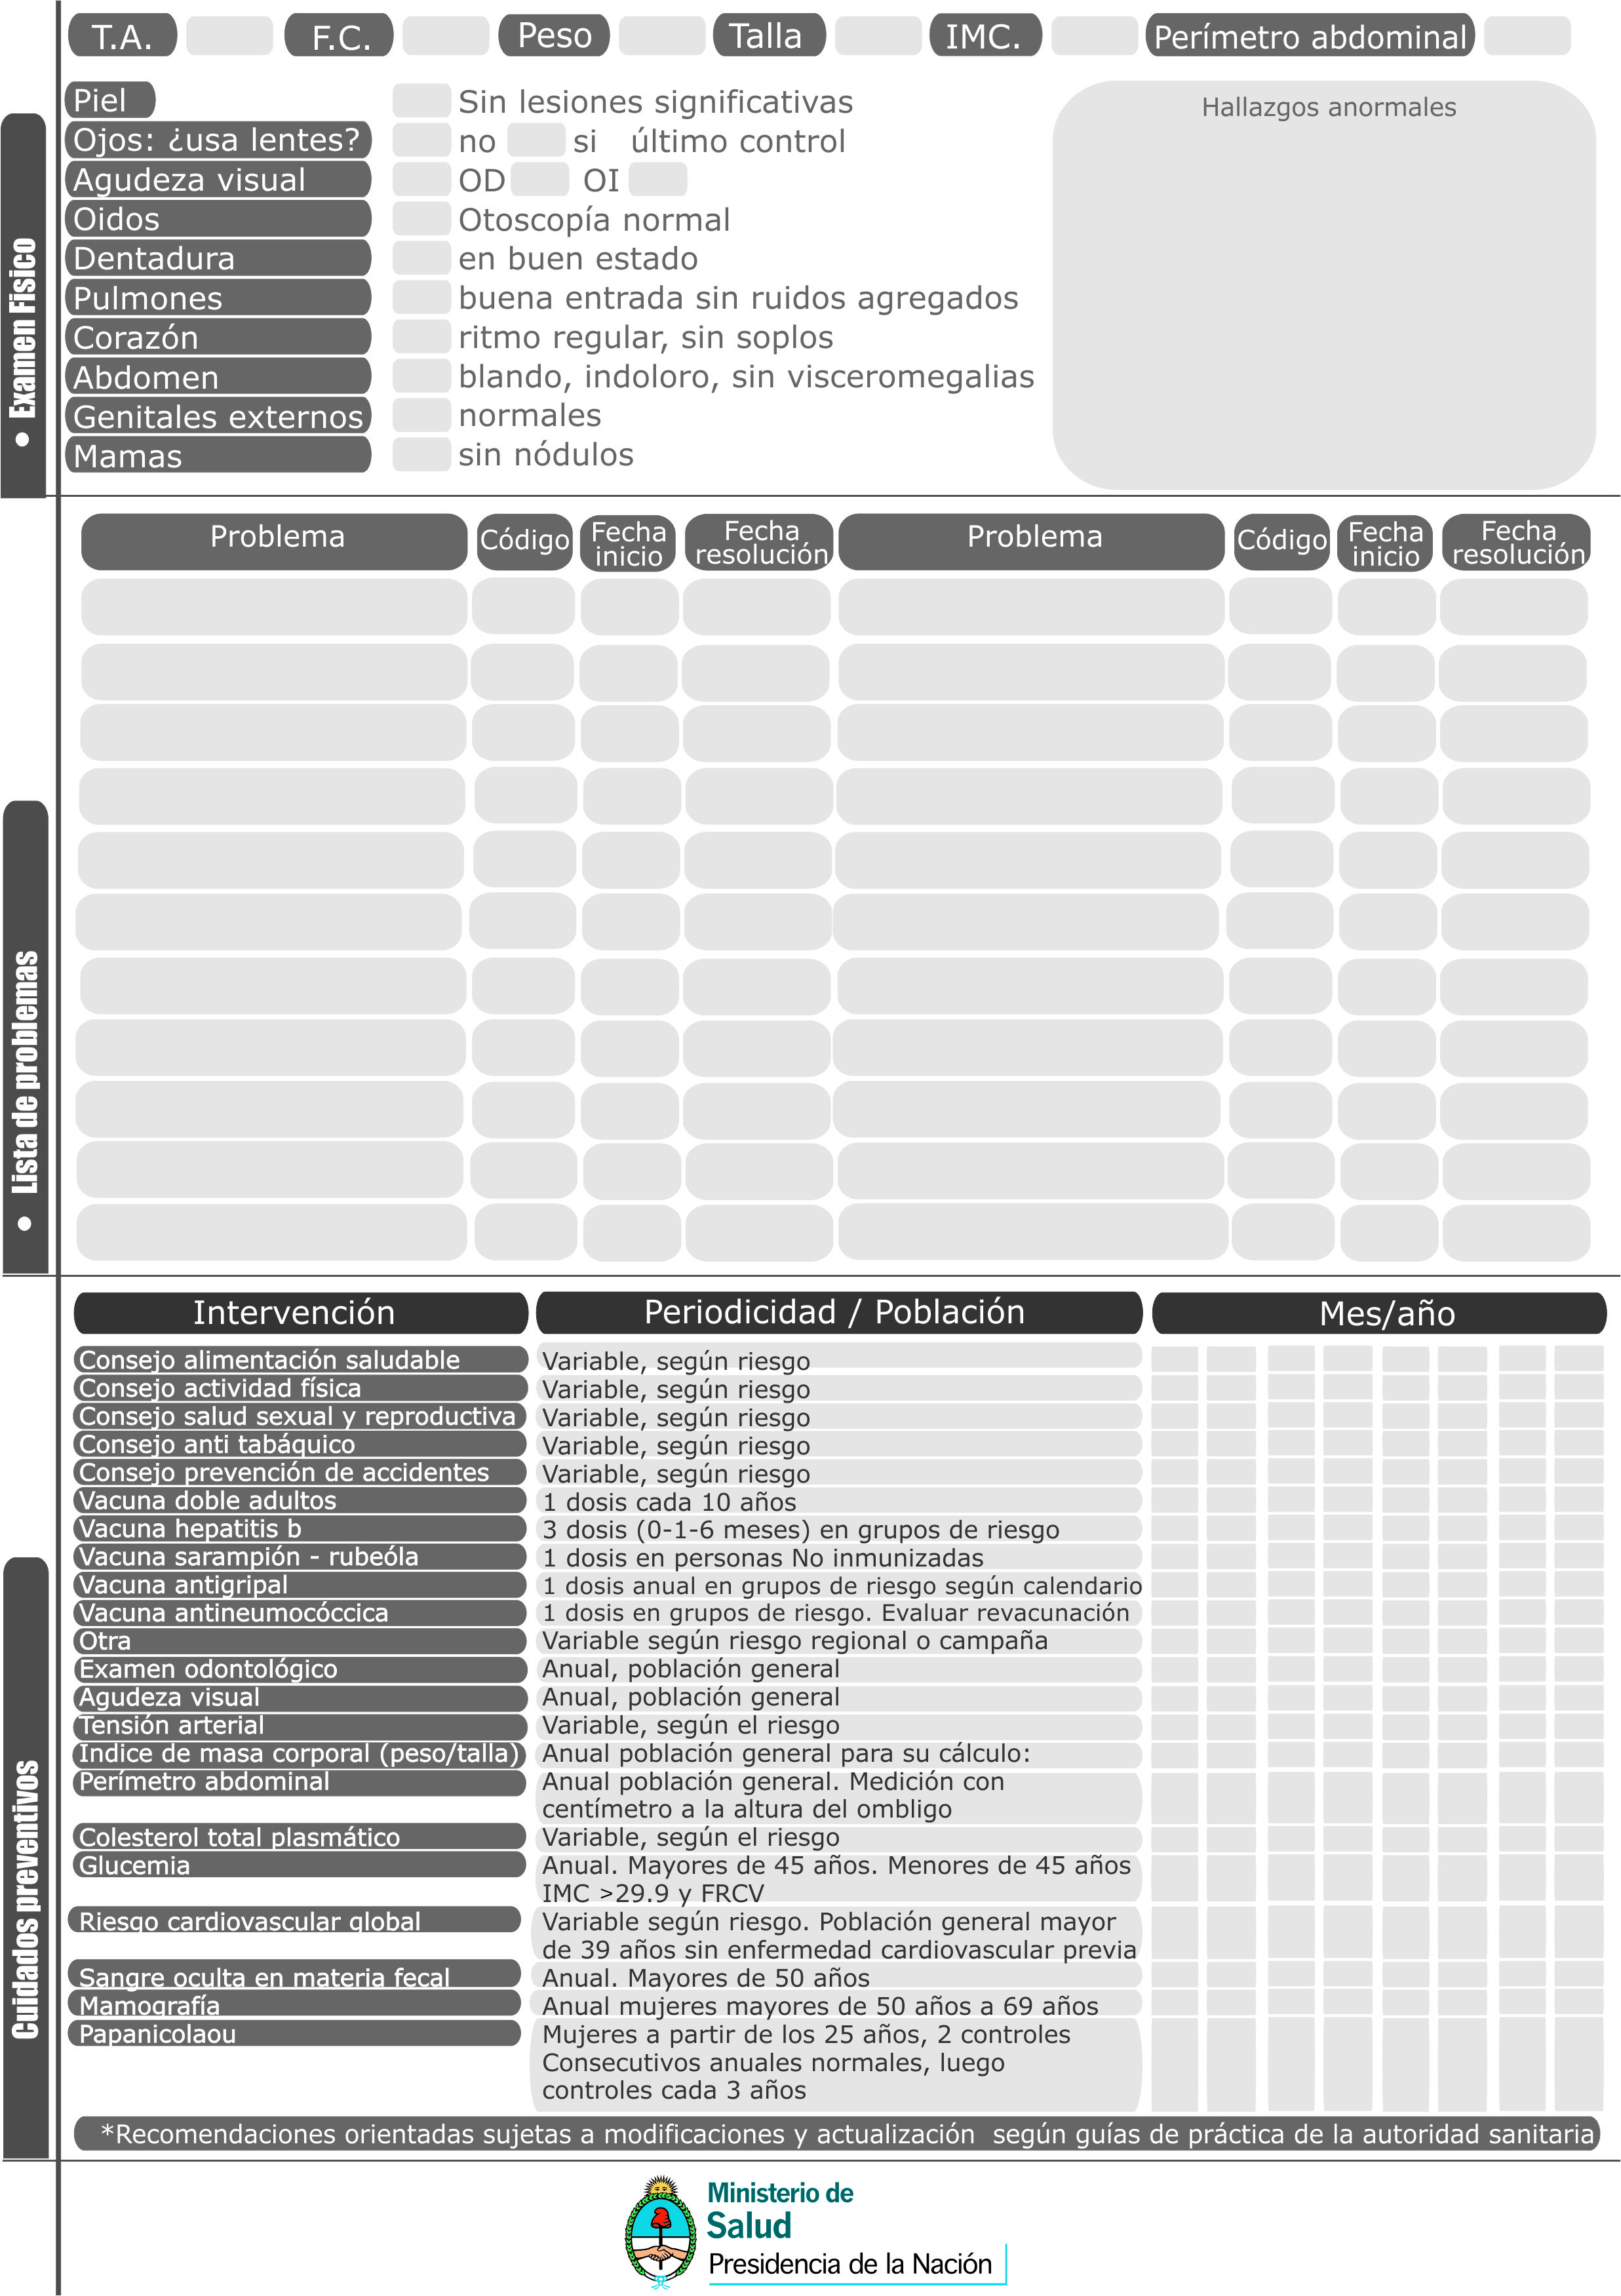
\includegraphics[scale=0.7]{resourse/historia-clinica-d.jpg}
    \caption{Modelo Historia Clinica Ministerio de Salud de La Nacion Pag 2}
    \label{fig:07}
\end{figure}

\section{Problemas del Sistema Actual}


\subsection{Almacenamiento}
 A medida que crece el numero pacientes y la informacion que va
anexando a cada Archivo se va necesitando mas espacio fisico para almancenar
dicha informacion. Por ello con el paso del tiempo las instalaciones dedicadas
a tal fin suelen verse colapsadas por los grandes volumenes de informacion que
deben manejar.\\[0.1cm]

\subsection{Busqueda y Localizacion}
La Busqueda de expedientes se puede agilizar un poco utilizando una buena organizacion,
el problema es que la mayoria de los edificios para tal fin, suelen estar saturados
por grandes volumenes de archivos fisicos, Por lo que encontrar un archivo requerido
suele ser una tarea costosa y lenta.\\[0.1cm]

\subsection{Deterioro}
En lo que hace a la conservación propiamente dicha, el combate de los
problemas habituales que se derivan de las condiciones climáticas, de la humedad,
de las plagas, del deterioro natural del papel, especialmente por su fabricación
con celulosa desde hace dos siglos, es una constante que, pese a sus avances,
no ha encontrado soluciones definitivas. Por ende, una preocupación común a los
archivos y bibliotecas, es encontrar remedios prácticos y asequibles para
asegurar la preservación de sus acervos. De lo anterior se desprende la
necesidad, en el nivel nacional, de procurar el establecimiento de políticas y
normas sobre conservación en las instituciones públicas y privadas dedicadas
a la protección del patrimonio.\\[0.1cm]

\subsection{Otros Poblemas}
Otros problemas que acarrean el uso de archivos fisicos son:

\begin{itemize}
    \item Pérdida, alteración o daño de documentos importantes
    \item Gasto excesivo en fotocopias
    \item Altos costos de personal para administrar, suplir, mantener y recuperar el archivo físico
    \item Costos asociados al transporte de documentos ya sea interna o externamente
    \item Costos asosiados al espacio físico requerido para su almacenamiento
    \item Falta de condiciones adecuadas para el almacenamiento de documentos como: ventilación, humedad, temperatura
    \item Falta de respaldo adecuado en caso de catastrofe como incendio, inundación o terremoto
\end{itemize}


\subsection{La Solucion Planteada}

Por ello este era un ecenario perfecto donde Es Necesario informatizar el
Actual Sistema, lo cual solucionaria los 2 principales problemas del mismo
que son el Excesivo espacio de almacenamiento y el lento trabajo de busqueda
ademas de:

\begin{itemize}
    \item Reducir costos de Personal Administrativo, ya que las busquedas y
    registro las hara el Sistema.
    \item Brindar la informacion de manera rapida en situaciones criticas que
    requieren un rapido accionar por parte del Medico.
   \item Disponibilidad En todo momento y cualquier lugar para consulta por
    parte de los Medicos ya que solo requerira disponer de un usuario y un
    ordenador con coneccion a Internet para poder consultar.
\end{itemize}

Es cierto que los sistemas informaticos sufren problemas de Almacenamiento, Busqueda
(en el caso de grandes volumenes de informacion) y deterioro por el paso del tiempo
Pero en este caso el primero se soluciona Agregando mas espacio de disco, cosa que
hoy en dia es algo relativamente barato a razon de 1 peso = 1 Gb. \footnote {Gb hace referencia a
Gigabyte que es una medida utilizada en informatica la cual normalmente hace referencia
a tama\~nos de almacenamiento.}  \\[0.1cm]

El problema de las busqueda no afecta mucho con la velocidad de los equipos
actuales se puede consultar bases de datos con millones de registro en unas
pocas milesimas de segundos dicho tiempo resulta impersectible para la persona
en la mayoria de las veses, en todo caso dependera de la implementacion y el
motor de bases de datos mas que de las prestaciones del hardware.\\[0.1cm]

En cuanto al deterioro, puede que con el tiempo los equipos de hardware
tales como discos duros fallen en algun momento, pero esto es salvable siempre y
cuando se realizen buenas practicas tales como implementar un sistemas de backup,
tambien replicacion de datos en caso de que se necesite alta disponibilidad de
la informacion que se almacena.\\[0.1cm]


\section{Gestion de Turnos}   

En lo que respecta a asignacion de turnos, el sistema actual en la mayoria de
los casos no ha tenido un mejor panorama en cuanto a implatancion de un software,
aunque ya en esta area existen algunas aplicaciones que intentan solucionar el
problema de manera mas o menos eficientes.\\[0.1cm]























